\section{Metodología}

\subsection{Recolección de datos}
En este proyecto, se emplearon datos de referencia obtenidos de artículos científicos, libros
especializados y modelos teóricos validados con el objetivo de definir las condiciones iniciales, los
parámetros físicos y las ecuaciones diferenciales ordinarias (EDO) que modelan el comportamiento de
un sistema simplificado de carga de baterías para vehículos eléctricos. Se optó por utilizar un modelo
representativo de una sola malla, lo que permitió reducir la complejidad del sistema original y
enfocarse en los componentes clave que determinan el proceso de carga, como el comportamiento del
capacitor, la resistencia interna y los elementos del convertidor.

Para la determinación de parámetros eléctricos fundamentales, se recurrió a los estudios realizados por
Sainz y Balcells (2011), quienes llevaron a cabo mediciones experimentales centradas en la
mitigación de corrientes armónicas en cargadores de baterías para vehículos eléctricos. Dichas
mediciones proporcionaron valores de referencia para la resistencia interna de la batería (\(R_{bat}\)) y la
capacitancia del sistema (\(C\)), parámetros esenciales para la formulación del modelo eléctrico del
circuito.

Asimismo, se consideraron los aportes de Cittanti, Mandrile y Bojoi (2021), quienes realizaron una
optimización del diseño de filtros LCL trifásicos destinados a la carga rápida de baterías. Esta
referencia fue crucial para establecer valores representativos de la resistencia equivalente (\(R_x\)) y de la
inductancia en la topología del sistema, contribuyendo a definir con mayor precisión los elementos
pasivos del circuito.

Además, el trabajo de Zhang, Wang y Li (2021) sobre convertidores boost con corrección del factor
de potencia permitió incorporar una perspectiva adicional sobre el comportamiento dinámico del
sistema de conversión, facilitando la validación de los parámetros del convertidor y asegurando que el
modelo matemático simplificado conserve coherencia con los dispositivos reales empleados en
procesos de carga.

En ausencia de datos experimentales propios, se generaron datos sintéticos a partir de los modelos
teóricos referenciados, complementados con soluciones analíticas reportadas en la literatura. Estos
datos permitieron avanzar con la simulación y análisis del sistema, garantizando la continuidad del
estudio bajo un enfoque metodológico riguroso.

\subsection{Análisis de datos}
Los datos recolectados se procesaron cuidadosamente para establecer las condiciones iniciales del
sistema y validar los resultados obtenidos. Se empleó un enfoque metodológico estructurado, que
abarca desde la formulación de la ecuación diferencial ordinaria (EDO) hasta la obtención de los
resultados numéricos, permitiendo una comparación de estos con soluciones analíticas conocidas o
datos de referencia. A continuación, se describe de manera detallada el proceso seguido para el
análisis de los datos:

\subsubsection*{Establecimiento de las condiciones iniciales:}
Los parámetros iniciales del sistema fueron establecidos utilizando los datos de referencia
provenientes de artículos científicos y modelos teóricos validados. Entre estos parámetros se
incluyeron:

\begin{itemize}
	\item \textbf{Resistencia interna de la batería (\(R_{bat}\)):} Determinada a partir de los estudios de Sainz y Balcells (2011) sobre la mitigación de armónicos en cargadores de baterías para vehículos eléctricos.

	\item \textbf{Capacitancia (\(C\)):} Parámetro que define la capacidad del sistema para almacenar energía, basado en las mediciones de Cittanti et al. (2021) sobre el diseño de filtros LCL trifásicos.

	\item \textbf{Resistencia equivalente del sistema (\(R_x\)):} Determinada por los valores encontrados en la optimización de filtros LCL.

	\item \textbf{Inductancia (\(L\)):} Tomada de los parámetros definidos por Cittanti et al. (2021) para el diseño de sistemas de carga rápida.
\end{itemize}

\subsubsection*{Formulación de la ecuación diferencial ordinaria (EDO):}
Con los parámetros definidos, se formuló la ecuación diferencial que describe el
comportamiento dinámico del sistema de carga de baterías. Está EDO modela la variación de
la carga almacenada en el capacitor en función del tiempo. La ecuación general que describe
este sistema es:

\[
	(R_{bat} + R_x + R_c) \cdot \frac{dq(t)}{dt} + \frac{q(t)}{C} = V_0 \sin(\omega t)
\]

Donde:
\begin{itemize}
	\item \(q(t)\) es la carga almacenada en el capacitor en el tiempo \(t\),
	\item \(V_0\) es el voltaje de entrada del sistema (proveniente de la batería),
	\item \(\omega\) es la frecuencia de la señal de entrada,
	\item \(R_{bat}\), \(R_x\) y \(R_c\) son las resistencias involucradas en el sistema.
\end{itemize}

Esta EDO representa un sistema de primer orden, y su solución es clave para entender el
comportamiento dinámico de la carga.

\subsubsection*{Simulación numérica:}
La simulación numérica es una de las herramientas fundamentales para resolver las
ecuaciones diferenciales y obtener los resultados que permitan evaluar el comportamiento
dinámico del sistema. En este caso, se utilizará la Transformada de Laplace y la función de
transferencia para resolver la ecuación diferencial ordinaria (EDO) que describe el
comportamiento del sistema de carga de baterías en el tiempo.

\paragraph*{Transformada de Laplace y Función de Transferencia:}
La Transformada de Laplace es una técnica matemática esencial para resolver
ecuaciones diferenciales en sistemas lineales, convirtiendo ecuaciones diferenciales
en ecuaciones algebraicas. Este paso simplifica significativamente el proceso de
análisis de sistemas dinámicos. En este caso, la ecuación diferencial del sistema de
carga se transformará del dominio del tiempo al dominio de Laplace.

La función de transferencia, derivada de la EDO, describe la relación entre la entrada
y la salida del sistema, en este caso, entre el voltaje de entrada y la carga almacenada
en el capacitor. La función de transferencia permite modelar cómo los filtros
electrónicos afectan la señal de entrada y mitigan los armónicos en el sistema de
carga.

\subsubsection*{Pasos en la Simulación:}
\begin{enumerate}
	\item \textbf{Transformación de la EDO al Dominio de Laplace:}
	      \begin{itemize}
		      \item La ecuación diferencial del sistema de carga es:
		            \[
			            (R_{bat} + R_x + R_c) \cdot \frac{dq(t)}{dt} + \frac{q(t)}{C} = V_0 \sin(\omega t)
		            \]
		      \item Aplicamos la Transformada de Laplace a ambos lados de la ecuación. La derivada en el tiempo se convierte en una multiplicación de \(s\), el operador de Laplace:
		            \[
			            (R_{bat} + R_x + R_c)sQ(s) + \frac{Q(s)}{C} = \frac{V_0}{s^2 + \omega^2}
		            \]
		      \item Aquí, \(Q(s)\) es la transformada de \(q(t)\) en el dominio de Laplace.
	      \end{itemize}

	\item \textbf{Resolución para Función de Transferencia:}
	      \begin{itemize}
		      \item De la ecuación obtenida en Laplace, despejamos \(Q(s)\) para obtener la función de transferencia \(G(s)\), que relaciona la carga \(Q(s)\) con la entrada \(V_0 \sin(\omega t)\):
		            \[
			            Q(s) = \frac{V_0}{ (R_{bat} + R_x + R_c)s + \frac{1}{C}} + \frac{1}{(s^2 + \omega^2)}
		            \]
		      \item La función de transferencia \(G(s)\) es crucial para entender cómo el sistema responde a diferentes entradas y cómo los armónicos son mitigados.
	      \end{itemize}

	\item \textbf{Validación de los Resultados:}
	      \begin{itemize}
		      \item Los resultados obtenidos de la simulación serán comparados con soluciones analíticas o datos experimentales de referencia. Se espera que la simulación numérica proporcione una respuesta precisa y coherente con los datos de referencia.
	      \end{itemize}
\end{enumerate}

\subsubsection*{Diagrama de flujo metodológico:}
Para garantizar la claridad y la trazabilidad de cada paso, se elaboró un diagrama de flujo que
describe el proceso metodológico desde la formulación de la EDO hasta la obtención de los
resultados (Anexo 1). Este diagrama incluye los siguientes pasos:
\begin{enumerate}
	\item \textbf{Recolección de datos:} Obtención de los parámetros iniciales y condiciones del sistema como \(R_{bat}\), \(R_x\), \(C\), etc.
	\item \textbf{Formulación de la EDO:} Determinación de la ecuación diferencial que describe el sistema de carga.
	\item \textbf{Simulación numérica:} Aplicación de métodos numéricos para obtener la solución temporal de la EDO.
	\item \textbf{Análisis de resultados:} Evaluación de los resultados obtenidos a partir de la simulación numérica.
	\item \textbf{Comparación con soluciones analíticas:} Validación de los resultados obtenidos mediante la comparación con soluciones analíticas o datos de referencia.
\end{enumerate}

\subsection{Justificación de la elección del enfoque analítico}
La resolución analítica de las ecuaciones diferenciales ordinarias (EDOs) se ha seleccionado como
enfoque principal para el análisis del sistema de carga de baterías, particularmente en el modelado del
convertidor boost, debido a varias razones clave que garantizan la precisión y adecuación del modelo
a este tipo de problema. A continuación, se detallan las razones por las cuales este enfoque es
apropiado:

\subsubsection*{Precisión y Soluciones Exactas:}
Una de las principales ventajas de la resolución analítica de las EDOs es su capacidad para
proporcionar soluciones exactas. A diferencia de los enfoques numéricos, que solo aproximan
los resultados y pueden ser sensibles a errores de discretización, las soluciones analíticas
ofrecen una representación precisa y directa del comportamiento del sistema. En este caso, la
solución exacta de la ecuación diferencial permite entender cómo varían con el tiempo
variables clave como la carga almacenada en el capacitor, la corriente en los componentes del
sistema y el voltaje de entrada. Esta precisión es crucial, ya que proporciona una base
confiable sobre la cual se pueden realizar simulaciones numéricas y comparaciones con otros
modelos o datos experimentales. La capacidad de obtener soluciones exactas también es útil
para validar los resultados obtenidos mediante simulaciones, asegurando que las
aproximaciones numéricas se ajusten adecuadamente a la realidad del sistema.

\subsubsection*{Adecuación al Problema Planteado:}
El enfoque analítico es particularmente adecuado para este proyecto debido a que el modelo
simplificado de primer orden, en el cual se ha planteado el sistema de carga de baterías, es
tratado con facilidad mediante soluciones analíticas. Al emplear un modelo de primer orden,
las ecuaciones resultantes se mantienen relativamente simples y no requieren la complejidad
computacional que implicaría el uso de métodos numéricos más avanzados, como los
métodos de elementos finitos o simulaciones basadas en grandes sistemas no lineales. La
viabilidad de las soluciones analíticas en este contexto facilita la comprensión del
comportamiento fundamental del sistema sin necesidad de recurrir a simulaciones pesadas, lo
cual es especialmente importante cuando se busca una primera aproximación o comprensión
del sistema sin introducir incertidumbres adicionales propias de los métodos numéricos.

\subsubsection*{Comprensión Profunda del Sistema:}
El enfoque analítico también permite una comprensión profunda del comportamiento
dinámico del sistema. Las soluciones exactas proporcionan información detallada sobre cómo
las variables del sistema interactúan entre sí y cómo pequeñas perturbaciones, como las
variaciones en el voltaje de entrada o los cambios en la resistencia interna de la batería,
afectan la dinámica del proceso de carga. Este conocimiento es esencial para optimizar los
filtros utilizados para mitigar los armónicos, ya que nos permite identificar las características
estables y transitorias del sistema. De hecho, las soluciones analíticas permiten estudiar tanto
el comportamiento estacionario (una vez que el sistema alcanza el equilibrio) como el
transitorio (durante las fases iniciales de la carga o cuando ocurren cambios en las
condiciones operativas). Esta visión es crucial para diseñar sistemas más eficientes y robustos.

\subsubsection*{Ventajas en Términos de Simulación y Optimización:}
Finalmente, la utilización de un enfoque analítico no solo contribuye a la precisión y
comprensión del sistema, sino que también facilita la optimización. Las soluciones exactas
obtenidas permiten evaluar rápidamente el impacto de diferentes parámetros sobre el sistema,
como la resistencia interna de la batería, la capacitancia o la inductancia. Esto es
especialmente útil para probar diferentes configuraciones del convertidor boost sin la
necesidad de realizar múltiples simulaciones, ahorrando tiempo y recursos. Además, al tener
una solución exacta como referencia, se puede comprobar la precisión de los resultados
obtenidos mediante simulaciones numéricas y ajustar el modelo según sea necesario.

\subsection{Procedimiento analítico}
% === FIGURA 4 ===
\begin{figure}[h]
	\centering
	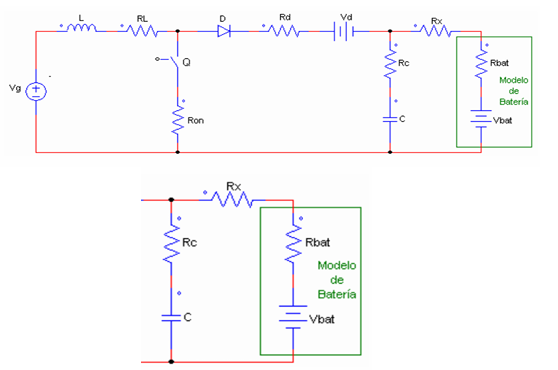
\includegraphics[width=0.8\textwidth]{4.png} % Reemplazar con ruta real
	\caption{Convertidor Boost con pérdidas en los elementos y modelo de batería.}
	\label{fig:procedimiento}
\end{figure}

El procedimiento analítico para resolver las ecuaciones diferenciales ordinarias (EDOs) que modelan
el comportamiento del sistema de carga de baterías para vehículos eléctricos se llevó a cabo en varias
etapas utilizando técnicas matemáticas bien establecidas, como separación de variables, coeficientes
indeterminados, y la Transformada de Laplace. A continuación, se describe cada uno de los pasos,
ilustrando cómo se aplica a la ecuación diferencial que describe el sistema.

\subsubsection*{Planteamiento del Modelo y la Ecuación Diferencial}
El sistema de carga de baterías está representada por un circuito que incluye tres resistencias
\(R_{bat}\), \(R_x\) y \(R_c\), un condensador \(C\), y una fuente de voltaje sinusoidal \(V_0 \sin(\omega t)\), como se
muestra en la siguiente ecuación diferencial:

\[
	(R_{bat} + R_x + R_c) \cdot \frac{dq(t)}{dt} + \frac{q(t)}{C} = V_0 \sin(\omega t)
\]

Definiciones:
\begin{itemize}
	\item \(q(t)\) → Es la carga almacenada en el condensador.
	\item \(C\) → Es la capacitancia del condensador.
	\item \(V_0\) → Es la tensión de la fuente de voltaje de la batería.
	\item \(\omega\) → Es la frecuencia de la señal sinusoidal.
	\item \(R_{bat}\), \(R_x\), \(R_c\) → Resistencias en el circuito.
\end{itemize}

Esta ecuación es de primer orden, lo que implica que la carga \(q(t)\) depende de su derivada
con respecto al tiempo.

\subsubsection*{Solución homogénea / transitoria}
Para abordar la solución homogénea de la ecuación diferencial, primero debemos eliminar el
término sinusoidal de la ecuación original, lo que da lugar a la siguiente forma simplificada:

\[
	(R_{bat} + R_x + R_c) \cdot \frac{dq(t)}{dt} + \frac{q(t)}{C} = 0
\]

Este es un sistema lineal de primer orden con coeficientes constantes, que corresponde a una
ecuación diferencial homogénea. El objetivo es encontrar la carga \(q(t)\) en función del tiempo
\(t\), que es la variable dependiente. Esta ecuación describe cómo la carga almacenada en el
condensador disminuye con el tiempo debido a las resistencias del circuito.

\paragraph*{Método de Separación de Variables:}
Dado que esta es una ecuación diferencial de primer orden y lineal, utilizamos el
método de separación de variables, el cual consiste en reorganizar la ecuación para
que las variables dependiente \(q(t)\) y la independiente \(t\) se encuentren en lados
opuestos de la ecuación.

La ecuación original se puede escribir de la siguiente forma:

\[
	\frac{dq(t)}{dt} = -\frac{(R_{bat} + R_x + R_c)}{C} \cdot q(t)
\]

Ahora, separamos las variables, llevando \(q(t)\) a un lado y \(dt\) al otro:

\[
	\frac{1}{q(t)} dq(t) = -\frac{(R_{bat} + R_x + R_c)}{C} dt
\]

Integrando ambos lados, tenemos:

\[
	\int \frac{1}{q(t)} dq(t) = -\int \frac{(R_{bat} + R_x + R_c)}{C} dt
\]

\[
	\ln |q(t)| = -\frac{(R_{bat} + R_x + R_c)}{C} \cdot t  + A
\]

Donde \(A\) es una constante de integración que se determinará mediante las condiciones
iniciales. Exponenciando ambos lados de la ecuación para despejar \(q_h(t)\):

\[
	q_h(t) = Ae^{-\frac{(R_{bat} + R_x + R_c)}{C} \cdot t}
\]

Está es la solución homogénea \(q_h(t)\) de la ecuación diferencial. El término exponencial
describe el comportamiento de la carga almacenada en el condensador en
el tiempo, que decae exponencialmente con una constante de tiempo \(\tau\), dado por:

\[
	\tau = C(R_{bat} + R_x + R_c)
\]

Donde \(\tau\) es la constante de tiempo del circuito, que determina la rapidez con la que la
carga decae. La constante \(A\) se determina a partir de las condiciones iniciales del
sistema.

Obteniendo la solución transitoria / homogénea:

\[
	q_h(t) = A e^{-\frac{t}{\tau}} \quad
\]

\subsubsection*{Solución particular / estacionaria}
Dado que el voltaje de entrada es de naturaleza sinusoidal, se busca una solución particular de
la forma:

\[
	q_p(t) = V_0\sin(\omega t)
\]

Donde:
\begin{itemize}
	\item \(q_p(t)\) → Es la carga almacenada en el condensador debido a la entrada sinusoidal.
	\item \(V_0\) → Es la amplitud del voltaje de entrada.
	\item \(\omega\) → Es la frecuencia de la señal sinusoidal.
\end{itemize}

\paragraph*{Método de Coeficientes Indeterminados}
Para resolver esta ecuación particular, aplicamos el método de coeficientes indeterminados.
Este método es adecuado cuando la solución incluye términos sinusoidales, como en este
caso.

En el método de coeficientes indeterminados, asumimos que la solución particular \( q_p(t) \)
tendrá la forma:

\[
	q_p(\omega t) = B \sin(\omega t) + C \cos(\omega t)
\]

\[
	q'_p(t) = B\omega \cos(\omega t) - C\omega \sin(\omega t)
\]

Al substituir esta forma en la ecuación diferencial homogénea, se obtiene el siguiente sistema
de ecuaciones para la carga en el circuito:

\[
	(R_{bat} + R_x + R_c) \cdot \frac{dq(t)}{dt} + \frac{q(t)}{C} = V_0 \sin(\omega t)
\]

Sustituyendo la forma de \( q_p(t) \) y su derivada:

\[
	(R_{bat} + R_x + R_c)(B\omega \cos(\omega t) - C\omega \sin(\omega t)) + \frac{B \sin(\omega t) + C \cos(\omega t)}{C} = V_0 \sin(\omega t)
\]

Ahora comparamos los coeficientes de \( \sin(\omega t) \) y \( \cos(\omega t) \) en ambos lados de la ecuación. La
ecuación en el lado derecho tiene solo \( \sin(\omega t) \), por lo que el coeficiente de \( \cos(\omega t) \) debe ser
igual a cero en el lado izquierdo. Esto nos da dos ecuaciones:

\begin{itemize}
	\item Coeficiente de \( \sin(\omega t) \):
	      \[
		      (R_{bat} + R_x + R_c)(-C\omega) + \frac{B}{C} = V_0
	      \]

	\item Coeficiente de \( \cos(\omega t) \):
	      \[
		      (R_{bat} + R_x + R_c) B\omega + \frac{C}{C} = 0
	      \]
\end{itemize}

Resolución de Constantes \( B \) y \( C \), de la segunda ecuación obtenemos:

\[
	(R_{bat} + R_x + R_c) B\omega + 1 = 0
\]

De aquí podemos despejar \( B \):

\[
	B = -\frac{1}{(R_{bat} + R_x + R_c) \omega}
\]

Sustituyendo \( B \) en la primera ecuación:

\[
	(R_{bat} + R_x + R_c)(-C\omega) +  \frac{\frac{-1}{(R_{bat} + R_x + R_c) \omega}}{C}  = V_0
\]

Finalmente, la solución particular \( q_p(t) \) es la suma de las funciones sinusoidales con las
constantes \( B \) y \( C \) determinadas.

\subsubsection*{Solución general:}
La solución general del sistema es la combinación de la solución homogénea y la particular,
es decir:

\[
	q(t) = q_h(t) + q_p(t)
\]

Esto da como resultado una expresión general que describe el comportamiento de la carga a lo
largo del tiempo.

Las condiciones iniciales juegan un papel crucial en la resolución de la ecuación, ya que
determinan los valores de las constantes de integración. En este caso, la condición inicial será
\(q(0) = 0\), lo que indica que al inicio del proceso (cuando \(t = 0\)), el capacitor está
completamente descargado. Esta condición permite obtener una solución particular que se
ajusta a la realidad del sistema desde su inicio.

La solución homogénea es:

\[
	q_h(t) = A e^{-\frac{t}{\tau}}
\]

La solución particular es:

\[
	q_p(\omega t) = B \sin(\omega t) + C \cos(\omega t)
\]

% Reemplazando en \(t = 0\), obtenemos:
%
% \[
%     q(0) = 0 = A e^{0} + B \sin(0) + C \cos(0)
% \]
%
% \[
%     0 = A + C
% \]
%
% Teniendo como resultado que \(C = -A\)

Entonces la solución general nos queda de la siguiente forma:

\[
	q(t) = A e^{-\frac{t}{\tau}} + B \sin(\omega t) + C \cos(\omega t)
\]

\subsection{Limitaciones del enfoque}
El enfoque analítico utilizado para resolver las ecuaciones diferenciales ordinarias (EDOs) en este
proyecto tiene ciertas limitaciones, especialmente cuando se enfrenta a sistemas no lineales o
condiciones de contorno complejas. A continuación, se identifican las principales limitaciones y se
discute cómo estas pueden afectar los resultados, proponiendo posibles soluciones y aproximaciones.

\subsubsection*{Dificultad para Resolver EDOs No Lineales}
Una de las limitaciones más destacadas del enfoque analítico es la dificultad para resolver
EDOs no lineales. En sistemas donde los componentes presentan comportamientos no
lineales, como los diodos, transistores, o cargas no lineales en los convertidores, las
equaciones diferenciales correspondientes no pueden ser resueltas de manera exacta mediante
métodos analíticos tradicionales. Según Carvajal Carreño et al. (2011), la no linealidad en
sistemas eléctricos generan ecuaciones que no tienen una solución cerrada sencilla, lo que
limita la capacidad de aplicar directamente un enfoque analítico para obtener respuestas
precisas.

\paragraph*{Impacto en los Resultados:}
La imposibilidad de obtener soluciones exactas para sistemas no lineales implica que
se requieren soluciones aproximadas o el uso de métodos numéricos para tratar los
efectos no lineales, lo que puede introducir errores o incertidumbres en el análisis.
Cómo Carvajal Carreño et al. (2011) destacan, los modelos numéricos permiten
simular comportamientos complejos en estos sistemas, pero a costa de una mayor
carga computacional y de una mayor aproximación de los resultados, lo que podría
afectar la precisión del análisis.

\subsubsection*{Condiciones de Contorno Complejas}
El enfoque analítico también encuentra limitaciones cuando se trata de condiciones de
contorno complejas o variables en el tiempo. En los sistemas eléctricos de carga de baterías,
las condiciones de contorno pueden cambiar según el tiempo, la temperatura u otros factores
dinámicos, lo cual complica aún más la resolución analítica. En particular, cuando se analizan
circuitos acoplados o sistemas con retroalimentación, las ecuaciones resultantes tienden a ser
más complejas y difíciles de manejar analíticamente.

\subsubsection*{Simplificaciones y Aproximaciones Teóricas}
Para poder abordar la complejidad de estos sistemas, es común hacer ciertas simplificaciones
o aproximaciones teóricas. Algunas de estas aproximaciones incluyen:

\begin{itemize}
	\item \textbf{Linealización de sistemas no lineales:} Se puede aproximar un sistema no lineal por un sistema lineal en un rango específico de operación, utilizando técnicas como el método de Taylor para aproximar la ecuación alrededor de un punto de operación específico.

	\item \textbf{Modelo de primer orden:} En muchos casos, se puede simplificar un sistema complejo a un modelo de primer orden (como hemos hecho en este proyecto) que permita realizar un análisis simplificado sin perder la esencia del comportamiento dinámico del sistema.

	\item \textbf{Aproximaciones de componentes:} En algunos casos, los componentes electrónicos pueden ser modelados de manera aproximada. Por ejemplo, un diodo no siempre se puede modelar de manera precisa en todas sus características, por lo que se puede usar un modelo simplificado de resistencia en serie y resistencia en paralelo para representar su comportamiento.
\end{itemize}

\paragraph*{Impacto en los Resultados:}
Aunque las simplificaciones pueden facilitar la resolución de las ecuaciones,
introducen aproximaciones que pueden no reflejar completamente el comportamiento
real del sistema, lo que afecta la exactitud de los resultados. Si las condiciones
operativas del sistema se alejan de las condiciones ideales consideradas en el modelo,
la validez de los resultados podría verse comprometida. Como se menciona en el
artículo de Carvajal Carreño et al. (2011), las aproximaciones pueden ser útiles para
obtener una visión general, pero deben ser manejadas con precaución en sistemas
donde las variaciones dinámicas son significativas.

\subsubsection*{Soluciones Aproximadas vs. Exactas}
A menudo, se recurre a soluciones aproximadas cuando no es posible obtener una solución
exacta. Técnicas como las series de potencias o la expansión en series de Fourier son
ejemplos de cómo se pueden aproximar las soluciones en sistemas complejos. Sin embargo,
estas soluciones no proporcionan una visión exacta del comportamiento del sistema, sino una
aproximación que depende de cuántos términos se incluyan en la expansión.

\paragraph*{Impacto en los Resultados:}
Las soluciones aproximadas pueden ser útiles para obtener una estimación del
comportamiento general del sistema, pero no deben ser usadas como la única base
para el diseño de sistemas reales. La exactitud de las aproximaciones dependerá de
cuántos términos se incluyan en la expansión y de la naturaleza de los sistemas.
